\documentclass{article}

\usepackage{graphicx}
\usepackage{tikz}
\usepackage{tikzsymbols}
\usetikzlibrary{calc,patterns,shapes.geometric}
\pagestyle{empty}
\usepackage[margin=0pt]{geometry}
\geometry{papersize={14in,12in}}

\def\centerarc[#1](#2)(#3:#4:#5){\draw[#1] ($(#2)+({#5*cos(#3)},{#5*sin(#3)})$) arc (#3:#4:#5);}

\begin{document}
	\begin{figure}
		\centering
		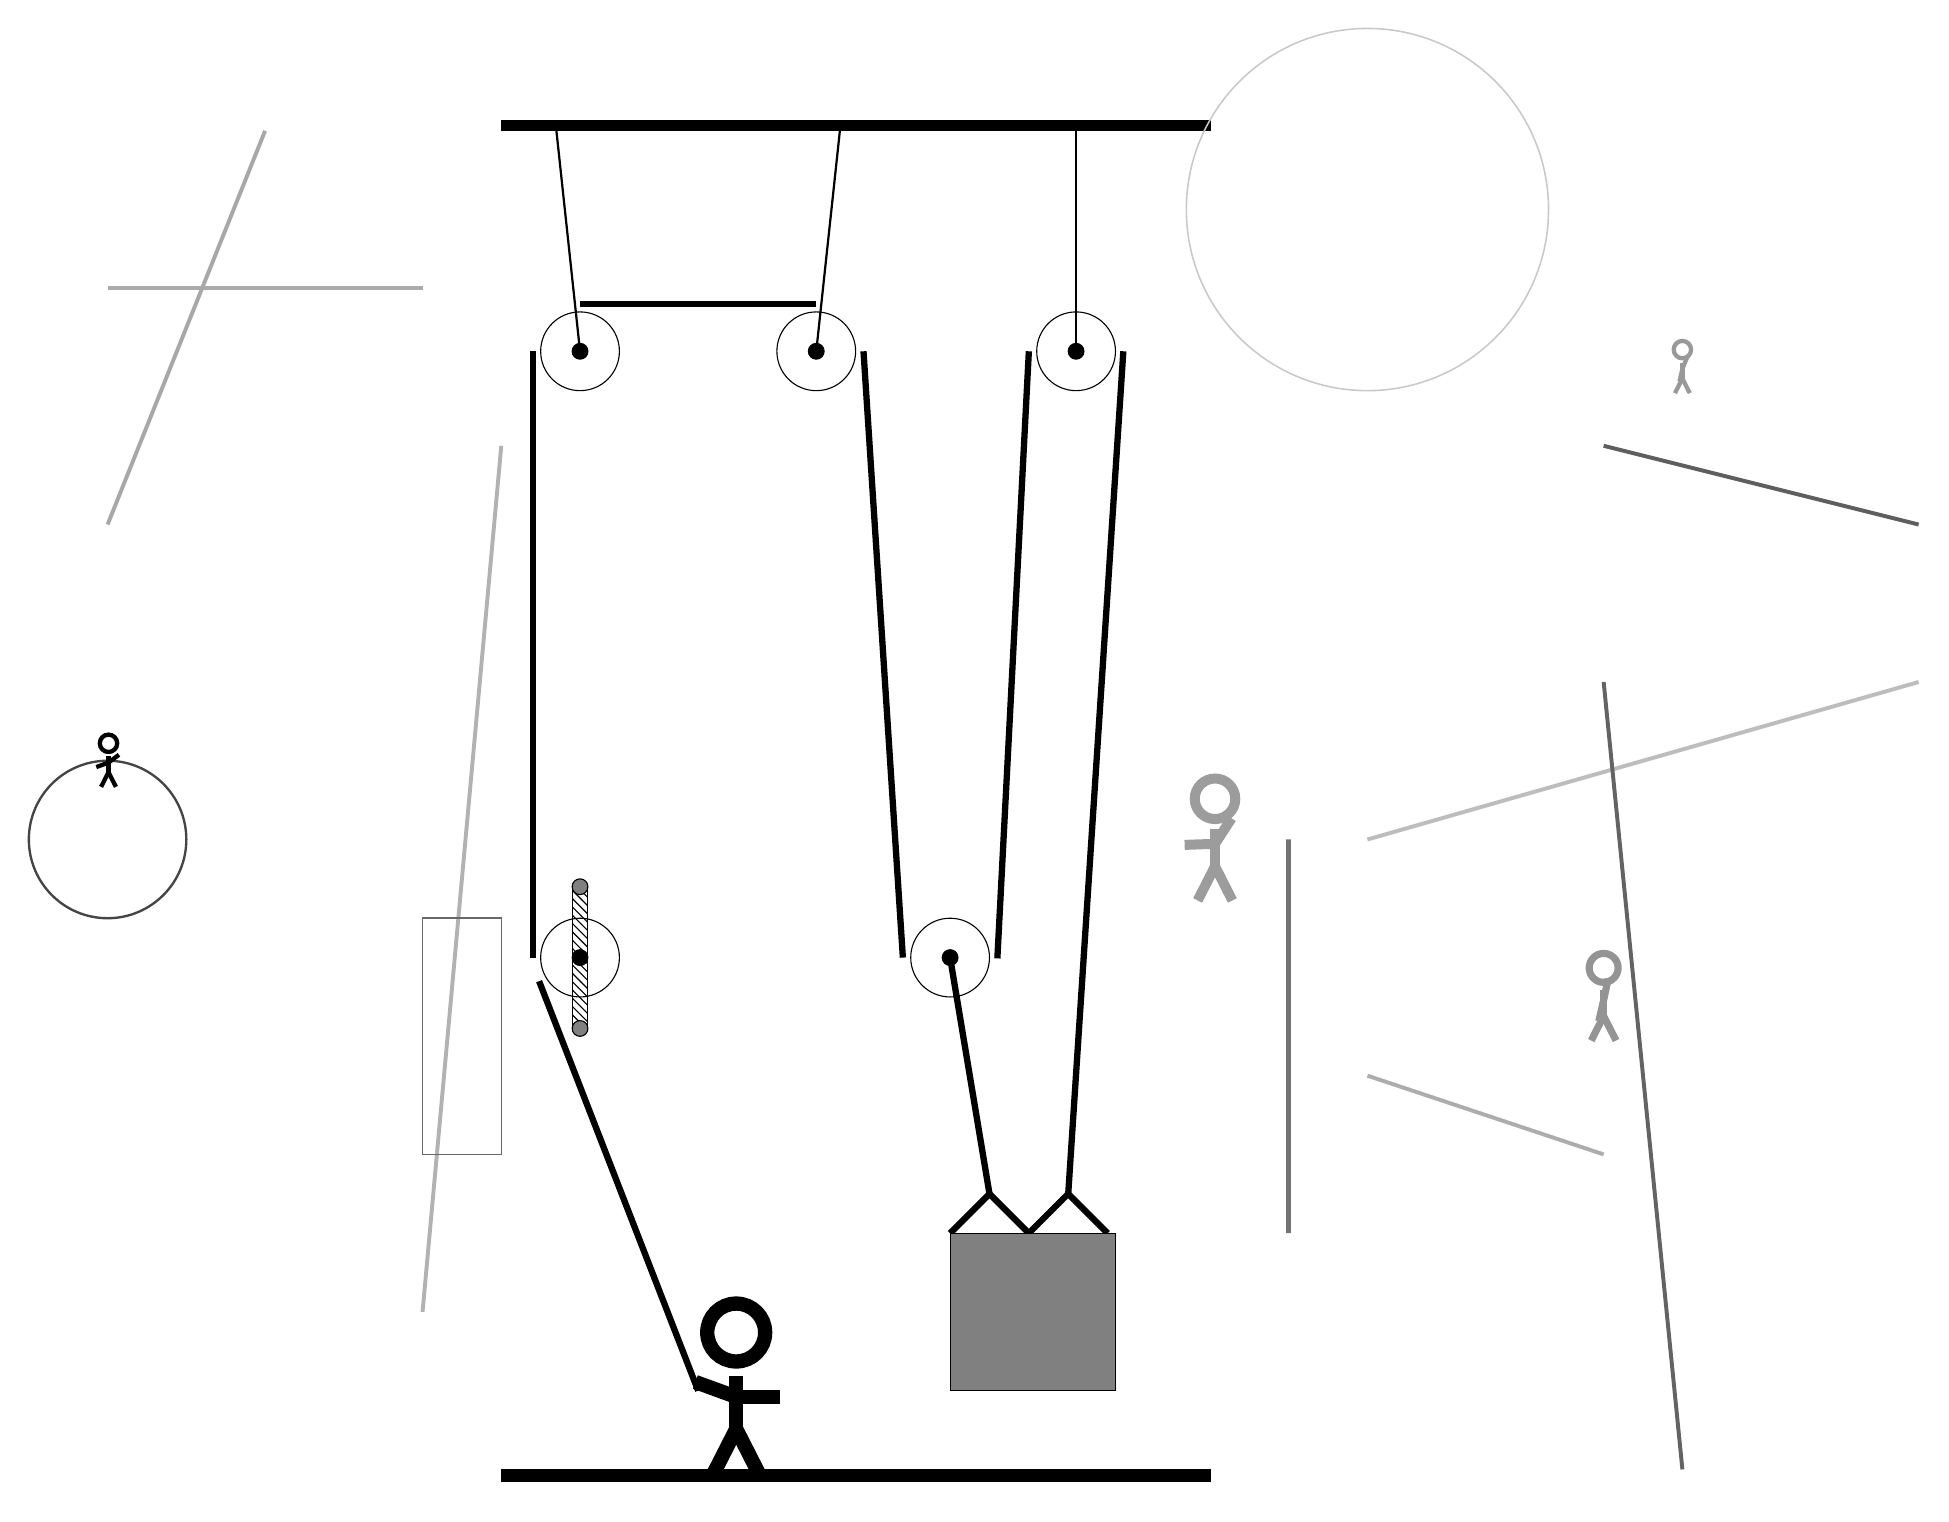
\begin{tikzpicture}
			%%%%% START %%%%%
			
			\draw[fill=black] (-3, 14) rectangle (6, 14.125);
			
			\draw (1, 11.2) circle (0.5);
			\draw[fill=black] (1, 11.2) circle (0.1);
			\draw[thick] (1, 11.2) -- (1.3, 14);
			
			\draw (4.3, 11.2) circle (0.5);
			\draw[fill=black] (4.3, 11.2) circle (0.1);
			\draw[thick] (4.3, 11.2) -- (4.3, 14);
			
			\draw (2.7, 3.5) circle (0.5);
			\draw[fill=black] (2.7, 3.5) circle (0.1);
			
			\draw[line width=0.8mm]  (2.7, 0) -- (3.2, 0.5) -- (3.7, 0) -- (4.2, 0.5) -- (4.7, 0);
			\draw[fill=black!50] (2.7, 0) rectangle (4.8, -2);
			
			\draw (-2, 11.2) circle (0.5);
			\draw[fill=black] (-2, 11.2) circle (0.1);
			\draw[thick] (-2, 11.2) -- (-2.3, 14);
			
			\draw (-2, 3.5) circle (0.5);
			\draw[fill=black] (-2, 3.5) circle (0.1);
			\draw[pattern=north west lines, pattern color=black] (-2.1, 4.4) rectangle (-1.9, 2.6);
			\draw[fill=black!50] (-2, 4.4) circle (0.1);
			\draw[fill=black!50] (-2, 2.6) circle (0.1);
			
			\draw[line width=0.8mm](-0.5, -2) -- (-2.5196, 3.2);
			\centerarc[line width=0.8mm](-2, 3.5)(180:210:0.6);
			\draw[line width=0.8mm](-2.6, 3.5) -- (-2.6, 11.2);
			\centerarc[line width=0.8mm](-2, 11.2)(90:180:0.6);
			
			\draw[line width=0.5mm, color=black!26](8, 5) -- (15, 7);
			
			\draw[line width=0.5mm, color=black!30](-4, -1) -- (-3, 10);
			\node[line width=0.3mm, color=black!42] at (11, 3) {\Strichmaxerl[5][77][78]};
			\draw [line width=0.3mm, color=black!73](-8, 5) circle (1.0);
			\node[line width=0.3mm, color=black!40] at (12, 11) {\Strichmaxerl[3][77][68]};
			
			\draw[line width=0.5mm, color=black!33](-8, 12) -- (-4, 12);
			
			\draw[line width=0.5mm, color=black!63](11, 10) -- (15, 9);
			\node[line width=0.7mm, color=black!100] at (-8, 6) {\Strichmaxerl[3][20][37]};
			\draw[line width=0.5mm, color=black!32](8, 2) -- (11, 1);
			\draw[line width=0.7mm, color=black!55] (7, 0) rectangle (7, 5);
			\draw[line width=0.5mm, color=black!61](11, 7) -- (12, -3);
			\node[line width=0.3mm, color=black!39] at (6, 5) {\Strichmaxerl[7][2][57]};
			\draw[line width=0.5mm, color=black!34](-8, 9) -- (-6, 14);
			
			\draw[line width=0.2mm, color=black!59] (-3, 4) rectangle (-4, 1);
			\draw [line width=0.2mm, color=black!21](8, 13) circle (2.3);
			
			\draw[line width=0.8mm](-2, 11.8) -- (1, 11.8);
			\centerarc[line width=0.8mm](1, 11.2)(0:90:0.6);
			\draw[line width=0.8mm](1.6, 11.2) -- (2.1, 3.5);
			\centerarc[line width=0.8mm](2.7, 3.5)(180:370:0.6);
			\draw[line width=0.8mm] (3.3, 3.49) -- (3.7, 11.2);
			\centerarc[line width=0.8mm](4.3, 11.2)(0:180:0.6);
			\draw[line width=0.8mm](4.2, 0.5) -- (4.9, 11.2);
			\draw[line width=0.8mm] (3.2, 0.5) -- (2.7, 3.5);
			
			\node at (0, -2) {\Strichmaxerl[10][-20][0]};
			
			\draw[fill=black] (-3, -3) rectangle (6, -3.15);
			
			%%%%% END %%%%%
		\end{tikzpicture}
	\end{figure}	
\end{document}